\cotefile{156-5}
\scanpage{2}
\mspage{1}
\margin{GF V}
% slanted
\margin{\uline{Algèbre} des \uline{figures}}
\uline{\unsure{Sorite} ensembliste}. \quad (14.6.86)

Soient $L$ un, $\unsure{\mathscr{L}|\mathcal{L}}\subset\unsure{\mathcal{P}|\mathscr{P}}(L)$ ens de parties de $L$. Posons
\[
|\mathscr{L}|=\deleted{\unsure{\mathscr{L}}}\bigcup_{A\in\mathscr{L}}A
\]
et pour $A\in\mathscr{L}$
\[
\partial A=\bigcup_{\substack{B\in\mathscr{L}\\B\subset A}}B,\qquad A^\circ=A\setminus\partial A
\]

% slanted
\margin{\unsure{Voir} variante ``indexée'' \uline{formellement} \uline{plus forte}, voir GF \uline{VIII}, \unsure{pg|p} 37....}
\uline{Proposition 1} Les conditions suivantes sont équivalentes :

$1^\circ)$ Pour tout $x\in L$, \deleted{\unsure{dans|dans l'} l'ens $\mathscr{L}_x$ des} \inserted{l'ensemble}
\[
\mathscr{L}_x=\{A\in\mathscr{L}\mid x\in A\}
\]
admet un plus petit élément, (noté $A(x)$).

$2^\circ)$ \deleted{\unsure{Pour}}On a les deux conditions

\[
\alpha)\ \forall A,B\in\mathscr{L},\quad\text{on a}\quad
 A\cap B=\bigcup_{\substack{C\in\mathscr{L}\\C\subset A\cap B}}C
\]
$\beta)$ $\forall x\in\mathscr{L}$, il existe un élément \uline{minimal} de $\mathscr{L}_x$ i.e. un $A\in\mathscr{L}$ tel que $x\in A^\circ$ -- i.e.
\[
\bigcup_{A\in\mathscr{L}}A^\circ=\unsure{(\mathscr{L})|\lvert\mathscr{L}\rvert}.
\]

$3^\circ)$ On a les \deleted{deux}\inserted{trois} conditions suivantes

(où \deleted{\unsure{\ensuremath{\mathscr{L}'}}} on a posé
\[
\mathscr{L}'=\{A\in\mathscr{L}\mid A^\circ\ne\varnothing\}
\]
$\gamma)$ La famille $\{A^\circ\}_{A\in\mathscr{L}'}$ forme une \uline{partition} de $|\mathscr{L}|$, i.e. $\forall x\in\unsure{\lvert\mathscr{L})|\lvert\mathscr{L}\rvert}$, \deleted{\unsure{\ensuremath{\exists!}}} existe un \uline{unique} $A\in\mathscr{L}'$ tel que $x\in A^\circ$, i.e.
\[
\bigcup_{A\in\mathscr{L}'} A^\circ=|\mathscr{L}|\quad\text{et}\quad
(A,B\in\mathscr{L}^{\unsure{*|\prime}},\ A^\circ\cap B^\circ\ne\varnothing)\Rightarrow(A=B)
\]

\margin{NB On \unsure{peut remplacer} $\delta,\unsure{\eta|\varepsilon}$ par $(\delta')$ $\forall A\in\mathscr{L}$, on a $A=\displaystyle\bigcup_{\substack{B\in\mathscr{L}\\B\subset A}}B^\circ$}
\[
\left\{\begin{aligned}
\delta)&\quad \deleted{\unsure{\text{Tout}|\forall A}}\,\forall A\in\mathscr{L},\quad A\ \text{est saturé dans }|\mathscr{L}|\\
 &\quad\text{pour la relation d'équivalence précédente.}\\
\eta)&\quad\text{Si } A,B\in\mathscr{L},\quad A^\circ\subset B\ \text{et }\
 \underset{\text{i.e. } A\in\mathscr{L}'}{\underbrace{A^\circ\ne\varnothing}}\ \Rightarrow A\subset B
\end{aligned}\right.
\]
\scanpage{3}
\mspage{2}
\uline{Dém}

$1^\circ\Rightarrow 2^\circ$ \quad Supposons $1^\circ$, \deleted{\unsure{on}}Prouvons $\alpha)$ et $\beta)$

$\alpha)$ Soit $x\in A\cap B$, donc $A(x)\subset A$, $A(x)\subset B$, donc
\[
 x\in C\subset A\cap B\qquad\text{d'où}\qquad A\cap B=
 \bigcup_{\substack{C\in\unsure{\mathscr{L}|\mathcal{L}}\\C\subset A,B}}C
\]

$\beta)$ trivial

$2^\circ)\unsure{=|\Rightarrow}3^\circ)$ \quad Prouvons $\gamma)\,\text{et})\ \delta),\unsure{\eta|\varepsilon})$

$\gamma)$ On sait $\displaystyle\bigcup_{A\in\mathscr{L}'}A^\circ=\bigcup_{A\in\mathscr{L}}A^\circ=|\mathscr{L}|$ par $\beta)$, prouvons que $A,B\in\mathscr{L},\ A^\circ\cap B^\circ\ne\varnothing\Rightarrow A=B$. Soit $x\in A^\circ\cap B^\circ$. Prouvons $A=B$ il suffit de prouver que $x\in A^\circ$ \deleted{$\Rightarrow A$ plus \unsure{pet|pet.}} \unsure{i.e.|ie.} $A$ minimal dans $\mathscr{L}_x$, implique que $A$ est un plus petit élément de $\mathscr{L}_x$. Soit $B\in\deleted{\unsure{B_x}}\mathscr{L}_x$, donc $x\in\deleted{\unsure{A^\circ}}B\deleted{\unsure{{}_x}}$ \deleted{\unsure{et}} $\Rightarrow$ $x\in A^\circ\cap B\subset\unsure{A'|A}\cap B\underset{\alpha}{=}\displaystyle\bigcup_{\substack{C\in\mathscr{L}\\C\subset A,B}} C$,
Comme $x\in C$, par le \unsure{car.} minimal de $A$ on a $C=A$, \unsure{comme|donc} $C\subset B$ on a $A\subset B$, OK.

$\delta)$ Soit $A\in\mathscr{L}$, $x\in A$, \deleted{prouvons que $A(x)^{\unsure{\circ}} \unsure{\subset|\in} A$} \deleted{i.e. $B\unsure{\subset|\in}$} \inserted{considérons} l'unique $B\in\mathscr{L}'$ tel que $x\in B^\circ$, il faut prouver que $B^\circ\subset A$, or on vient de voir que \deleted{$B$ est \unsure{i|:}} $x\in B^\circ\Rightarrow B$ est plus petit élément dans $\mathscr{L}_x$ ; donc on a $\deleted{\unsure{B=}}B\subset A$, donc $B^\circ\subset A$, qed.

\inserted{$\eta)$ A été vu \unsure{au|en} cours de route : si $x\in A^\circ$, $x\in B$, alors $A\subset B$.}

$3^\circ\Rightarrow1^\circ$. \quad On suppose $\gamma)$ et $\delta)$ prouvons $1^\circ)$. Soit $x\in|\mathscr{L}|$, par $\gamma)$ $x$ appartient à un unique $A^\circ$ \unsure{*|x|,} $(A\in\mathscr{L}')$, prouvons que $A$ est plus petit \unsure{él} de $\mathscr{L}_x$. Soit $B\in\mathscr{L}$ tel que $x\in B$, il faut prouver $A\subset B$. \deleted{\unsure{Comme}} Par $\delta$ $B$ est saturé donc $x\in B$, $x\in A^\circ\Rightarrow A^\circ\subset B$. \deleted{Il faut donc prouver que $A^\circ$} Par $\eta$, on a $A\subset B$\unsure{,|.}
\scanpage{4}
\mspage{3}
\uline{\unsure{Remarque|Remarques}} \deleted{Si \unsure{de|dans} \unsure{\textcircled{1}} $2^\circ)$,} \inserted{$1^\circ)$} La condition $\beta)$ de $2^\circ$ est automatique si $\unsure{\mathscr{L}|\mathcal{L}}$ fini, plus \unsure{gén.} si $\mathscr{L}$ est ``artinien'' pour $\subset$, i.e. s'il n'existe pas de suite str. décroissante d'éléments de $\mathscr{L}$
\[
 A_1\supset A_2\supset\ldots
\]
Si par contre $\mathscr{L}$ est réduit à \deleted{\unsure{une telle}} \inserted{\unsure{l'ens des}} termes d'une telle suite, \deleted{\unsure{alors} \illegible{1}} alors $\alpha$ est satisfaite mais non $\beta$ si $\displaystyle\bigcap A_{\unsure{i|n}}\ne\varnothing$.

$2^\circ)$ Dans $3^\circ$, \deleted{il suffit de supposer} la \unsure{condition} $\unsure{\eta|\varepsilon})$ n'est pas surabondante,
\[
\left\{\begin{aligned}
 &\deleted{\displaystyle\bigcup_{A\in\mathscr{L}'}A^\circ=|\mathscr{L}|}\\
 &\deleted{\displaystyle\forall A\in\mathscr{L},\ \text{on a } A=\bigcup_{\substack{B\in\mathscr{L}\\\text{t.q. }B^\circ\subset A}}B^\circ}
\end{aligned}\right.
\]
comme on voit dans l'exemple suivant
\[
\deleted{\mathscr{L}=\{A,B,C,D\}\quad\text{\deleted{\unsure{de}} \unsure{sur|où}}\ L=\{x,y,z,t\}}
\]
\figure{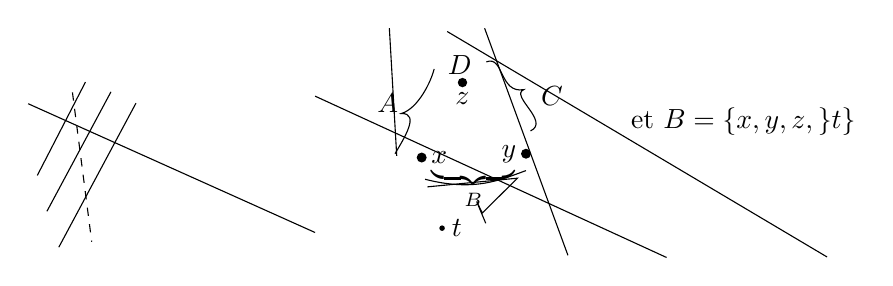
\begin{tikzpicture}[x=0.72cm,y=0.69cm,baseline]
\node at (2.05,2.18) {$\deleted{D}$};
\fill (2.10,1.85) circle (1.7pt) node[below] {$\deleted{z}$};
\fill (1.38,0.47) circle (1.8pt) node[right] {$\deleted{x}$};
\fill (3.22,0.54) circle (1.8pt) node[left] {$\deleted{y}$};
\fill (1.74,-0.83) circle (1pt) node[right] {$\deleted{t}$};
\node at (0.78,1.47) {$\deleted{A}$}; \node at (3.68,1.60) {$\deleted{C}$};
\draw (1.60,2.10) .. controls (1.55,1.88) and (1.32,1.37) .. (1.02,1.28)
 .. controls (1.36,1.29) and (1.06,.81) .. (.91,.54);
\draw (2.52,2.23) .. controls (2.83,2.36) and (2.75,1.64) .. (3.18,1.72)
 .. controls (2.93,1.61) and (3.65,1.13) .. (3.30,.96);
\node at (2.29,-.10) {$\deleted{\unsure{\underbrace{\hspace{3em}}_{B}}}$};
\draw (1.44,.07) .. controls (2.30,-.16) and (2.75,.05) .. (3.22,.23);
\draw (1.48,-.07)--(3.07,.09)--(2.45,-.55)--(2.35,-.34)--(2.51,-.74);
\node[right] at (4.9,1.14) {\deleted{et $B=\{x,y,z,\deleted{\unsure{\}}}\unsure{t}\}$}};
\draw[thin] (-4.55,1.86)--(-5.40,.14) (-4.10,1.68)--(-5.23,-.52) (-3.66,1.47)--(-5.02,-1.18);
\draw[dashed,thin] (-4.78,1.67)--(-4.44,-1.08);
\draw[thin] (-5.56,1.46)--(-.5,-.91);
\draw[thin] (-.5,1.60)--(5.70,-1.37); \draw[thin] (1.83,2.79)--(8.53,-1.36);
\draw[thin] (.81,2.85)--(.94,.50); \draw[thin] (2.49,2.85)--(3.96,-1.33);
\end{tikzpicture}}
\[
\deleted{A^\circ=\{x\},\ C^\circ=\{y\},\ D^\circ=\{z\},\ B^\circ=
\deleted{\unsure{\varnothing|\{z\}}}\{t\}}
\]
% slanted
\margin{Exemple \unsure{idiot} -- mais voir contre\unsure{xemple|exemple} correct (avec \unsure{I} \uline{infini}) GF \uline{VIII}, p\unsure{ges|ages} 44,45.}
\[
\begin{aligned}
 &\deleted{\mathscr{L}=\{A,B,C,D\}\qquad\text{avec}}\\
 &\deleted{A\cap C=D,\quad\deleted{\unsure{D|A}\unsure{\subset|=}\,B}}
\end{aligned}
\]
\diagram{\begin{tikzcd}[ampersand replacement=\&,row sep=1.1em,column sep=1em]
 \& \deleted{D} \arrow[dl,no head,bend right=45,shorten <=2pt,shorten >=2pt] \arrow[dr,no head,bend right=48,shorten <=2pt,shorten >=2pt] \& \\
 \deleted{A} \& \& \deleted{C} \arrow[dl,no head,bend left=8] \\
 \& \deleted{\unsure{B}}\deleted{B} \&
\end{tikzcd}}
\deleted{donc}
\[
\begin{aligned}
 &\deleted{\deleted{A^\circ=A\setminus D,\ \unsure{t|1}}}\\
 &\deleted{D^\circ=D,\ A^\circ=A\setminus D,\ C^\circ=C\setminus D,\ B^\circ=B\setminus(A\cup C)}
\end{aligned}
\]
\deleted{\deleted{On a $A^\circ\subset B$} On a $A^\circ\subset B$ mais non pas $A\subset B$. Ici \deleted{$A^\circ$} tous les $X^\circ$ $(X\in\mathscr{L})$ sont non vides.}

\margin{\deleted{[\unsure{\ensuremath{\delta}|\ensuremath{\eta}} \unsure{et} si $A\in\mathscr{L}\Rightarrow A\ne\varnothing$ ??]}}
\uline{Définition} On dit que $\mathscr{L}$ est \uline{préadmissible}, si elle satisfait les conditions équivalentes $1^\circ,2^\circ,3^\circ$. \unsure{!} On dit qu'elle est \uline{admissible} si de plus
\scanpage{5}
\mspage{4}
\unsure{pour} \deleted{\unsure{le}}\unsure{tt|\ensuremath{\forall}} $A\in\unsure{\mathscr{L}|\mathcal{L}}$, on a $A^\circ\ne\varnothing$. (Donc l'ens d'indices de la partition de $3^\circ)\,\gamma$ est $\mathscr{L}$ lui-\unsure{\ensuremath{=}|m})

\deleted{\uline{Proposition 2} Soient $\mathscr{L},\Psi$ deux familles préadmissibles. Conditions équivalentes :}

% slanted
\margin{Souvent il est plus commode de dire que c'est un \uline{préordre} sur $S$ -- $I$ est \unsure{l'ens.} ordonné associé, $\unsure{R|\mathscr{R}}_{\mathscr{L}}$ la \unsure{rel.} \unsure{d'éq.} \unsure{d'équivalence|dite} \unsure{associée}, \unsure{pour|par} le \unsure{préordre|préordonné}. Les $A\in\mathscr{L}$ sont les parties fermées \uline{\unsure{irréd.}}}
% slanted
\margin{\uline{NB} \unsure{Se donner} une famille \uline{pré}admissible, c'est se donner un système comme dessus (\deleted{\unsure{qui corres}} \inserted{où} $I=\mathscr{L}'=\{A\in\mathscr{L}\mid A^\circ\ne\varnothing\}$) et de plus, un ens. \unsure{fini|fin.} \deleted{de \unsure{parti}} $\Psi$ de parties fermées de $I$ (\unsure{correspondant} aux éléments de $\mathscr{L}\setminus\mathscr{L}'$)}

Se donner \unsure{dans|sur} $L$ une famille admissible \inserted{$\mathscr{L}$} de parties, revient au $=$ que de se donner

a) Un ens ordonné $I$ \qquad (une copie conforme de $\mathscr{L}$)

b) Une partie $S$ de $L$ \qquad ($S=|\mathscr{L}|$)

c) Une application surjective $\unsure{\varphi|\phi}:S\unsure{\text{---}|\longrightarrow}I$ \quad ($x\mapsto A(x)$)

Prenant sur $I$ la top. associée à l'ordre (où les fermés sont les réunions quel\uline{conques} d'ens. $I_{\leq i}$, les ouverts les réunions quelc. d'ens $I_{\geq i}$) -- donc $\uline{\ensuremath{J\subset I}}$ est fermé ssi $\deleted{\unsure{\forall}}i\in J,\ j\leq i\Rightarrow j\in J$) et sur $S$ la top. image inverse (qui est aussi celle définie par le préordre induit de l'ordre de $I$ via $\varphi$), \deleted{les} on récupère $\deleted{\unsure{P}}\mathscr{L}$ comme
\[
 \mathscr{L}=\left\{\overline{\varphi^{-1}(i)}=\varphi^{-1}
 \bigl(\overline{\{i\}}=I_{\leq i}\bigr)\right\}_{i\in I}
\]
(indexation fidèle). Les parties fermées de $S$ sont les réunions quelconques \deleted{de} ``\unsure{strates} fermées'' i.e d'éléments de $A$, elles correspondent \deleted{\unsure{d|1} à \unsure{un|un*}}\inserted{\unsure{biuniv.}} aux parties fermées \inserted{$J$} de $I$ ($\unsure{\simeq|\cong}$ \deleted{de} $\mathscr{L}$), \inserted{par transp. inv. par $\varphi$} \deleted{les parties ouvertes sont les correspondants aux}
\[
\deleted{\unsure{X}}A_J=\bigcup_{i\unsure{\leq|\in}J}A_i
 =\underset{\substack{\text{si on identifie}\\I=\mathscr{L},\ \text{donc }J\subset\mathscr{L}}}{\bigcup_{A\in J} A}
 =\underbrace{\deleted{\unsure{\bigcup}}\bigsqcup_{i\in J}A_i^\circ}_{\substack{\text{réunion}\\\text{disjointe}\\\text{de parties}\\\text{non vides}}}
\]
\uuline{NB} \deleted{Si on regarde les}

De $=$, les parties ouvertes sont \unsure{celles} de
\scanpage{6}
\mspage{5}
la forme
\[
 \deleted{\unsure{X}}\unsure{A|X}_J=\bigcup_{i\in J}A_i^\circ={\unsure{\varphi|\phi}}^{-1}(J)
 \tag*{(1)}
\]
où $\deleted{\unsure{A}}J$ est une partie ouverte de $I$ (ou de $\unsure{\Phi|\Psi|\mathscr{L}}\simeq I$) (\deleted{\unsure{bien}} \unsure{sûr|non}, cette fois dans $\displaystyle\bigcup_{i\in J}$ il n'est pas question de remplacer $A_i^\circ$ par $A_i$ !). Les parties loc. fermées sont de \unsure{\ensuremath{=}|m} les
\[
 \deleted{\unsure{X}}A_J=\varphi^{-1}(J)=\bigcup_{i\in J}A_{\unsure{i}}^\circ
\]
où cette fois $J$ est une partie loc fermée de $I$, i.e. telles que
\[
 i\leq j\leq k,\quad i,k\in J\quad\Rightarrow\quad j\in J
 \tag*{$(*)$}
\]
(les $\deleted{\unsure{J|I}}I_{\geq i}$, $i\in J$, sont des ouvert de $I$ recouvrant $J$, et \deleted{\unsure{dans cet}}\inserted{pour un tel} ouvert, \deleted{$J$}\inserted{$J\cap I_{\geq i}$} est fermé \inserted{dans $I_{\geq i}$,} à cause de $(*)$, donc $J$ est bien loc. fermé si on a $(*)$, l'inv. étant encore plus évident \ldots)

\uline{NB} On peut aussi dire, \inserted{si $\unsure{\mathscr{L}|\mathcal{L}}$ fini,} que les $A^\circ$ $(A\in\mathscr{L})$ sont les \deleted{\unsure{at}} \unsure{fibres} de l'algèbre de Boole engendrée par les $A\in\mathscr{L}$ dans $\unsure{\mathcal{P}|\mathscr{P}}(S)$ $(S=|\mathscr{L}|)$. Les ens obtenus à partir des $A\in\mathscr{L}$, par réunions, intersections et \unsure{complémentaires|complémentations} dans $S=\unsure{\lvert\mathscr{L})|\lvert\mathscr{L}\rvert}$, sont exactement ceux saturés par la rel d'équiv. dans $S$ définie par les $\unsure{A^\circ|X^\circ}$ \unsure{i.e.|id.} celle définie par $\varphi$. Donc ils correspondent biuniv. aux parties quelc. de $I$, par la \unsure{forme|formule}
\[
 J\longmapsto A_J=\varphi^{-1}(J)=\bigcup_{i\in\unsure{J|\supset}}A_i^\circ .
\]
On \unsure{appelera|appellera} \unsure{ses|ces|les} ens \unsure{ainsi|aussi} les \uline{parties} $\mathscr{L}$-\uline{modérées} ou $\mathscr{L}$-\uline{constructibles} de $\mathscr{L}$.
\scanpage{7}
\mspage{6}
\unsure{``} \uline{Sous-famille} \inserted{(ou sous-ens)} \uline{admissible} d'un ens admissible $\unsure{\mathscr{L}|\mathcal{L}}\subset\unsure{\mathcal{P}|\mathscr{P}}(L)$ : par définition, c'est un $\Psi\subset\mathscr{L}$ qui est \uline{fermé} dans $\mathscr{L}$. Alors pour $A\in\Psi$, $\deleted{\unsure{\partial_{\mathscr{L}}A}}$ on a
\[
 \partial_{\Psi}A=\partial_{\mathscr{L}}A\quad\text{donc}\quad
 A^{\circ(\deleted{\mathscr{L}}\Psi)}=A^{\circ(\mathscr{L})},
\]
ce qui montre que $|\Psi|$ est une partie saturée de $|\mathscr{L}|$, pour la rel. d'équiv. $\deleted{\unsure{\mathscr{L}}}R_{\mathscr{L}}$ \unsure{\ensuremath{s=}|sur|\ensuremath{S=}} $|\mathscr{L}|$,
\deleted{La top. de $\Psi$ est induite}

En fait, avec les notations précédentes, on a
\[
 |\Psi|=A_\Psi
\]
\deleted{De \unsure{\ensuremath{=}|m}, il est évident que pour \unsure{ce|x}} Soit $x\in|\Psi|$, donc $\deleted{\unsure{A}}\exists A\in\Psi$ tel que $\unsure{a|x}\in A$, \deleted{$x\in|\Psi|\Rightarrow$} et \unsure{donc} $x\in A(x)\subset A$ (puisque $A(x)$ est le plus petit des éléments de $\mathscr{L}$ qui $\ni x$) donc $A(x)\in\Psi$ ($\Psi$ étant fermé). Donc $A(x)$ est aussi le plus petit élément \uline{de $\Psi$} qui contient $x$ :

\deleted{\unsure{Ain}} Ainsi, $\Psi$ est préadmissible, et de plus il est évident que il est admissible (les $A^{\circ\unsure{\Psi|(\Psi)}}\ne\varnothing$, d'après $A^{\circ(\Psi)}=A^{\circ\mathscr{L}}$).

\uline{Prop.} Soit $\mathscr{L}\subset\mathcal{P}(L)$ ens de parties admissible, et soit $\Psi\subset\mathcal{P}(L)$. Conditions équivalentes

a) $\Psi\subset\mathscr{L}$, et $\Psi$ est une partie fermée de $\mathscr{L}$

b) $\Psi\subset\mathscr{L}$, $\Psi$ est admissible, \inserted{$|\Psi|$ est saturé dans $|\mathscr{L}|$ pour $\unsure{R_{\Psi}|R_{\varphi}|R_{\mathscr{L}}}$,} et la relation d'équivalence \inserted{$R_\Psi$} \unsure{sur|de} $|\Psi|\subset|\mathscr{L}|$ définie par $\Psi$ est celle induite par $R_{\mathscr{L}}$\unsure{.}
\scanpage{8}
\mspage{7}
On vient de voir que $a)\unsure{\Rightarrow|=} b)$ prouvons l'inverse, supposons $b)$ prouvons $a)$ i.e. soient $A\in\Psi$, $B\in\unsure{\mathscr{L}|\mathcal{L}}$, $B\deleted{\unsure{\in}}\subset A$ prouvons $B\in\Psi$

Considérons $B^\circ$, on a $B^\circ\ne\varnothing$ ($\Psi$ adm.) et comme $R_\Psi=R_{\mathscr{L}}\lvert\deleted{\unsure{\mathcal{P}|B}}\Psi\rvert$ \inserted{\unsure{saturé|saturée}}, on a $B^\circ=C^\circ$ pour $C\in\deleted{\mathscr{L}}\Psi$ convenable, mais cela implique $\deleted{\unsure{C}}B=C$, donc $B\in\Psi$, qed.

On dit que $\Psi$ est une \uline{sous-famille} \uline{admissible}.

\uline{Scholie} Elles correspondent \inserted{(avec conservation des rel. d'ordre)} aux parties fermées de $\mathscr{L}$, ou de $|\mathscr{L}|$. \unsure{\ensuremath{\Rightarrow}|=}\,Elles sont \uline{stables} par $\cup$ et $\cap$ quelc. dans $|\mathscr{L}|$.

\uline{Proposition} Soient $\mathscr{L},\Psi\subset\unsure{\mathcal{P}|\mathscr{P}}(L)$ deux ens de parties admissibles. Conditions équiv.

a) $\mathscr{L}\cup\Psi$ est admissible, et $\mathscr{L},\Psi$ en sont \unsure{deux|des} sous-ens. admissibles (i.e. fermés)

\inserted{$\deleted{\unsure{a}}a')$ $\mathscr{L}$ et $\Psi$ sont \deleted{\unsure{deux}}sous-familles adm. d'une famille \inserted{adm.} $\Sigma$}
b) $\mathscr{L}\cap\Psi$ est $\mathscr{L}$-fermé dans $\unsure{\Phi|\mathscr{L}}$ et \inserted{$\Psi$-fermé} dans $\Psi$,
\[
 \text{et}\qquad |\mathscr{L}|\cap|\Psi|=|\mathscr{L}\cap\Psi|
\]
c) $|\mathscr{L}|\cap|\Psi|$ est $\mathscr{L}$-fermé dans $|\mathscr{L}|$ et \unsure{\ensuremath{\{}|,} $\Psi$-fermé dans $\Psi$, et \deleted{\unsure{toute} $A\in\mathscr{L}$ telle que} pour $A\subset|\mathscr{L}|\cap|\Psi|$, $A\in\mathscr{L}$ \deleted{de $\mathscr{L}$} ssi $\unsure{A|1}\in\Psi$, (i.e. ssi $A\in\mathscr{L}\cap\Psi$).

% slanted
\margin{Cf condition équiv. page 11 (\unsure{genre|sorte} d), ``strate par strate''}
\deleted{d) $\forall A\in\mathscr{L}, B\in\Psi$, on ait $\unsure{A}\ \mathscr{L}_{\unsure{\leq A|<A}}$ et $\Psi_{\unsure{\leq|<}}$}

$a')\Leftrightarrow a)$ évident par les sorites précédents de \unsure{\ensuremath{=}|m} que $a)$ implique $b)$ et $c)$. Reste à prouver $b\Rightarrow c$, $c\Rightarrow a$.

Prouvons d'abord $b\Rightarrow c$. Comme $|\mathscr{L}|\cap|\Psi|=\unsure{\lvert\mathscr{L}\cap\Psi)|\lvert\mathscr{L}\cap\Psi\rvert}$ par $b)$, et $\mathscr{L}\cap\Psi$ fermé dans $\mathscr{L}$ et
\scanpage{9}
\mspage{8}
fermé dans $\Psi$, il s'ensuit que $\lvert\unsure{\mathscr{L}|\mathcal{L}}\cap\Psi\rvert$ est fermé dans $\lvert\mathscr{L}\rvert$ et fermé dans $\lvert\Psi\rvert$\unsure{..|.} Soit $A\in\mathscr{L}$, $A\subset\lvert\mathscr{L}\rvert\cap\lvert\Psi\rvert=\lvert\unsure{\Phi|\mathscr{L}}\cap\Psi\rvert$, on a donc par le sorite préliminaire (comme $\mathscr{L}\cap\Psi$ fermé dans $\Psi$) que $A\subset\displaystyle\bigcup_{\deleted{\unsure{C}}B\in\mathscr{L}\cap\Psi}B$, cela implique \deleted{que $A\ \exists!$} (comme les $B$ dans $\mathscr{L}$) que $\exists\,B\in\mathscr{L}\cap\Psi$ tel que $A\subset B$.
\deleted{Appliquant le \unsure{\ensuremath{=}|m} raisonnement à $B$ (qui est $\subset\mathscr{L}\cap\Psi$ donc $\subset\lvert\Phi\cap\Psi\rvert=\lvert\mathscr{L}\rvert\cap\lvert\Psi\rvert$) on} Mais comme $\mathscr{L}\cap\Psi$ est \deleted{\unsure{f}}$\Psi$ fermé dans $\Psi$, on en conclut $A\in\Psi$, qed.

$c\Longrightarrow a$ \quad On suppose c), prouvons a).

$1^\circ)$ $\mathscr{L}\cup\Psi$ est admissible. Soit $x\in\lvert\mathscr{L}\cup\Psi\rvert=\lvert\mathscr{L}\rvert\cup\lvert\Psi\rvert$ \deleted{\inserted{Si $x$} soit $A(x)$ le plus} Si $x\in\lvert\mathscr{L}\rvert\cap\lvert\Psi\rvert$, soit $A(x)$ le plus petit élément de $\mathscr{L}$ tel que $x\in A(x)$, et \unsure{itout|itou}. $B(x)\in\Psi$ \unsure{..,|.,} $x\in B(x)$. Comme $T=\lvert\mathscr{L}\rvert\cap\lvert\Psi\rvert$ est $\mathscr{L}$-fermé dans $\lvert\mathscr{L}\rvert$, on a $A\deleted{\unsure{\in}}(x)\subset T$, et de $=$ $B(x)\subset T$. On doit donc avoir (par c) $A(x)\in\Psi$ ie \deleted{$A(x)\in\mathscr{L}\cap\Psi$, et} donc par définition de $B(x)$ on a $\deleted{\unsure{A}}B(x)\subset A(x)$, de $=$ $A(x)\subset B(x)$, \inserted{soit $\unsure{C|D}$}
\deleted{donc} \inserted{\unsure{donc}} Cela montre que $C$ est le plus petit élément de $\mathscr{L}\cup\Psi$ qui conti\deleted{\unsure{ennent|enne}}\inserted{\unsure{ent}} $x$. Il reste à prouver que si $A\in\mathscr{L}\cup\Psi$, alors \deleted{$A$ n'est \unsure{p|pas}} \[
 \bigcup_{\substack{B\in\mathscr{L}\cup\Psi\\B\subsetneq A}}B
 \ne\deleted{\unsure{C|B}}A^{\text{\deleted{\unsure{ce|car}}}} .
\] \deleted{Mais} Il \deleted{$A\in\mathscr{L}$, $\unsure{\Psi|B}$ \illegible{3} $B\subset A$} suffit pour ceci de prouver que \inserted{si \unsure{(p. ex.)|(p.ex)} $A\in\mathscr{L}$,} les $B$ en
